\subsection{Esecuzione dell'esperienza}

L'esecuzione dell'esperienza è molto semplice. Avevamo a nostra disposizione le seguenti diapositive:

\begin{itemize}
    \item{Diapositiva con fessure di larghezza nominale 160, 80, 40 e 20 micrometri.}
    \item{Diapositiva con 5 fili di spessore sconosciuto a cui abbiamo aggiunto un capello di uno dei membri del gruppo.}
    \item{Diapositiva con 2 fori di diametro ignoto.}
    \item{Diapositiva con 3 reticoli da 100, 300 e 600 fessure per millimetro.}
\end{itemize}

\begin{figure}[b!]
    \centering
    \begin{subfigure}[b]{0.3\textwidth}
        
\includegraphics[width=\textwidth]{f1.png}
        \caption{Filo o fessura}
        \label{fig:ff}
    \end{subfigure}%
    ~ %add desired spacing between images, e. g. ~, \quad, \qquad etc.
      %(or a blank line to force the subfigure onto a new line)
    \begin{subfigure}[b]{0.3\textwidth}
        
\includegraphics[width=\textwidth]{f2.png}
        \caption{Foro}
        \label{fig:foro}
    \end{subfigure}
    ~ %add desired spacing between images, e. g. ~, \quad, \qquad etc.
      %(or a blank line to force the subfigure onto a new line)
    \begin{subfigure}[b]{0.3\textwidth}
        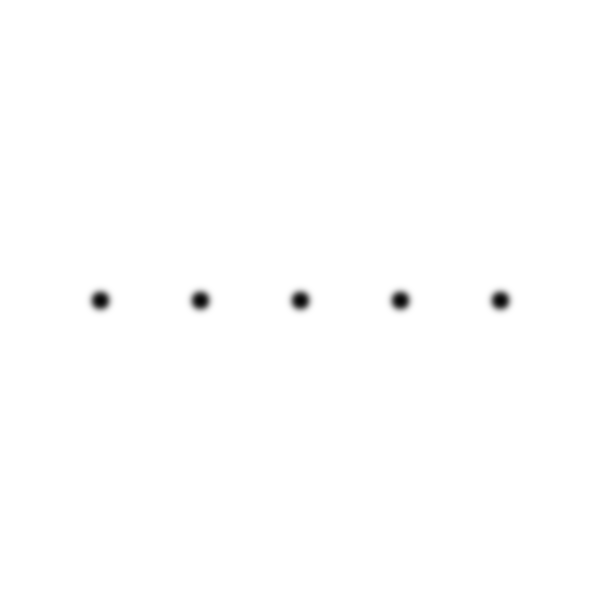
\includegraphics[width=\textwidth]{f3.png}
        \caption{Reticolo}
        \label{fig:ret}
    \end{subfigure}
    \caption{Figure di diffrazione generate da diversi tipi di ostacoli. Notare che, in maniera contro intuitiva,
        le aree nere sono quelle illuminate, mentre quelle bianche sono quelle che restano al buio. La figura nel caso di
        fili e fessure è identica grazie al principio di Babinet. Quando c'è un foro, invece la luce interferisce lungo
        tutte le direzioni e non solo nella direzione in cui la fessura è stretta, e genera una figura di diffrazione
        circolare. Il caso del reticolo è simile al caso della fenditura, solo che le fenditure sono molte, ed interferiscono
        in maniera diversa.}
    \label{fig:diff}
\end{figure}

Le misure sono state eseguite nel seguente modo. Per ogni diapositiva, abbiamo posto sul percorso del raggio laser ogniuno degli ostacoli
presenti sulla diapositiva, uno alla volta (ovviamente :-) ). Nel fare ciò, ci siamo presi la briga di controllare, alzando ed abbassando
la diapositiva, che la figura di diffrazione fosse la più pulita possibile. Questo significa trovare il luogo della fessura che ha i bordi
migliori. Dopodiché abbiamo incollato allo schermo una striscia di carta per annotare picchi di luce ed ombra. La distanza tra le tacche
è stata misurata con il calibro. Siccome la figura cambia a seconda dell'ostacolo abbiamo variato la procedura di misura come segue:

\begin{itemize}
    \item{Nel caso di fili e fessure la figura di diffrazione è lineare e presenta dei massimi e minimi larghi e ``sfuocati'' con un andamento
        sinusoidale (si veda Figura \ref{fig:ff}). Abbiamo segnato sulla carta i minimi di intensità, ovvero le parti dello schermo
        che restano al buio.}
    \item{Nel caso dei fori la figura di diffrazione è un cerchio centrale con vari anelli luminosi concentrici separati da
        zone scure (minimi di intensità, si veda Figura \ref{fig:foro}). Inoltre, a parte il centro ed il primo anello,
        la figura è molto debole e difficilmente
        percepibile ad occhio nudo. Poiché la misura del primo minimo è difficoltosa a causa della larghezza dello stesso, abbiamo segnato
        l'inizio e la fine del minimo e poi mediato i valori ottenuti.}
    \item{Nel caso dei reticoli di diffrazione la figura di interferenza presenta dei picchi molto luminosi e dei minimi molto larghi
            (In realtà ci sono anche dei minimi secondari, ma sono talmente deboli da non essere percepibili. Disegno in Figura \ref{fig:ret}).
            La misura dei minimi è quindi esclusa, per cui abbiamo misurato la separazione tra i massimi dello stesso ordine.
            Per i reticoli la misura è stata effettuata con entrambi i laser a nostra disposizione. Nei punti precedenti abbiamo
            usato esclusivamente il laser rosso.}
\end{itemize}

Le Tabelle \ref{tab:ff} e \ref{tab:foret} riportano tutti i dati misurati. Ci teniamo a far notare
che, sebbene molte misure siano state effettuate con il calibro e siano riportate anche le frazioni di millimetro,
l'incertezza di queste misure è molto più alta, a causa dello spessore delle tacche segnate sul foglio e a causa del
fatto che spesso erano storte e magari doppie. A nostro parere l'incertezza più appropiata è un incertezza di
risoluzione di 1 mm per le misure effettuate con il calibro, incertezza che abbiamo usato nei calcoli.
Le misure riguardanti i reticoli sono state effettuate con il metro a causa dell'intervallo di misurazione ampio. Anche in questo caso
l'incertezza di risoluzione è stata posta ad 1 mm, anche se forse si poteva portare fino a 2 mm.

\begin{table}[t!]
    \centering
    \footnotesize
    \begin{tabular}{c c c c | c c c c c c}
        \toprule
        \multicolumn{4}{c|}{Fessure [mm]} & \multicolumn{6}{c}{Fili [mm]}  \\
        \SI{160}{\micro\metre}& \SI{80}{\micro\metre}& \SI{40}{\micro\metre}& \SI{20}{\micro\metre}&
        Filo 1&  Filo 2&  Filo 3& Filo 4& Filo 5& Capello \\[1mm]
        \midrule
        12.65&     24.80&    48.40&   103.30& 34.50&    21.35&   17.50&  10.65&  3.05&   28.55  \\
        25.50&     49.25&    97.10&   209.80& 70.70&    42.15&   34.20&  21.15&  8.30&   56.00  \\
        37.75&     73.70&   146.75&   313.00& 104.60&   62.45&   51.40&  30.30&  14.00&  84.15  \\
        50.10&     98.90&   195.00&         & 149.20&   82.45&   67.90&  40.70&  21.10&  112.40 \\
        62.55&    124.10&   246.05&         & 174.95&   104.15&  85.30&  50.75&  28.00&  139.15 \\
        74.85&    148.40&&                  & 124.30&   101.90&  60.85&  34.40&       &         \\      
        88.25&&&                            & 144.90&   118.30&  71.00&  41.60&       &         \\
        100.15&&&                           &       &   135.65&  81.00&  48.25&       &         \\
        113.10&&&                           &       &        &       &   54.55&       &         \\
        125.70&&&                           &       &        &       &        &       &         \\
        \bottomrule
    \end{tabular}
    \caption{Distanza misurata tra i minimi dello stesso ordine nel caso della diapositiva con le fessure ed
        in quella con i fili. Il titolo delle colonne, nel caso delle fessure, si riferisce alla larghezza nominale delle fessure.
        Tutte le misure sono riportate in millimetri e sono state misurate con il calibro ventesimale. Tuttavia
        le cifre dopo la virgola sono molto incerte a causa della dimensione delle tacche sulla carta, e non dovrebbero
        essere considerate significative.}
    \label{tab:ff}
\end{table}

\begin{table}[b!]
    \centering
    \footnotesize
    \begin{tabular}{c c | c c c | c c c}
        \toprule
        \multicolumn{2}{c|}{Fori [mm]} & \multicolumn{6}{c}{Reticoli [mm]} \\[1mm]
        Foro 1 &      Foro 2 & R 100 &   R 300 &   R 600 & A 100 & A 300 & A 600\\
        \midrule
        63.50 &           32.75      & 198   &   597   &   1282  & 191   & 576   & 1232 \\
        65.00 &           30.25      & 399   &   1266  &         & 385   & 1218  &      \\
        64.00 &           29.50      & 640   &         &         & 584   &       &      \\
        63.50 &           30.00      &       &         &         &       &       &      \\
        \bottomrule
    \end{tabular}
    \caption{La tabella riporta i dati misurati per le diapositive con i fori e con i reticoli.
        Nel caso dei fori la figura di diffrazione è del tipo riportato in Figura \ref{fig:foro}
        ed i valori riportati sono alcuni diametri del primo minimo. Ogni valore è stato ottenuto mediando
        due dati misurati nel bordo interno e nel bordo esterno del minimo, poiché la misura diretta è risultata
        troppo arbitraria. Le misure sono state effettuate col calibro, ma le cifre dopo la virgola sono poco significative.
        I dati dei reticoli si riferiscono invece ai massimi di ordine uguale
        (primo ordine per la prima riga, secondo per la successiva, etc), poiché i minimi sono molto larghi.
        Le misure sono state effettuate colo metro poiché le distanze sono molto grandi. Nel titolo delle colonne R indica il laser
        rosso, A quello arancione, mentre il numero indica la densità di fessure per millimetro del reticolo. Le misure
        sono state effettuare per ogni reticolo con entrambi i laser. Tutte le misure sono in millimetri.}
    \label{tab:foret}
\end{table}

\subsection{Analisi dati}

L'analisi dati è divisa in 3 parti. Nella prima ci occupiamo di ottenere la dimensione degli ostacoli
che abbiamo messo sul percorso del raggio laser. La seconda si occupa di determinare la distanza
delle fessure dei reticoli, prendendo come dato in input la lunghezza d'onda del laser usato.
La procedura da usare per ricavare la dimensione di fenditure, fili e fori è differente da quella usata
per i reticoli, per motivi che chiariremo in seguito.
Nella terza parte ci proponiamo di rovesciare la situazione: vogliamo calcolare la lunghezza d'onda dei due
laser usati prendendo come input la dimensione delle fessure dei reticoli, riportate sugli stessi dal costruttore.

\begin{wrapfigure}{r}{52mm}
    \vspace{-5mm}
    \begin{center}
        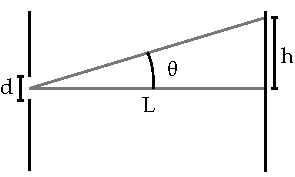
\includegraphics[width=48mm]{fen.pdf}
    \end{center}
    \vspace{-2mm}
\end{wrapfigure}

\subsubsection{Ostacoli vari}

Vogliamo calcolare la dimensione delle fenditure, dei fili e dei fori in esame.
La formula usata nell'analisi dati è la seguente:

\begin{equation}
    d = \frac{m\lambda}{\sin(\vartheta)}
    \label{eq:mindif}
\end{equation}

dove $d$ indica la larghezza della fenditura (si veda disegno a fianco),
$m \in \mathbb{Z} \setminus \{0\}$ indica l'ordine del minimo in questione,
$\lambda$ è la lunghezza d'onda della luce e $\vartheta$ è l'angolo che identifica
il minimo di ordine $m$ sullo schermo.

La formula si ottiene calcolando dove si trovano i minimi di intensità sullo schermo.
Quindi essa ci permette di ricavare $d$ se conosciamo la posizione di un qualsiasi minimo
della figura di diffrazione.

Durante l'esperimento abbiamo misurato la distanza tra minimi dello stesso ordine per i vari ostacoli.
Abbiamo quindi misurato la grandezza $2h$, i cui valori sono riportati nelle Tabelle \ref{tab:ff} e \ref{tab:foret}.
Nella (\ref{eq:mindif}) abbiamo bisogno di $\sin(\vartheta)$. Poiché gli angoli in gioco sono molto piccoli, tutti minori
di 6 gradi, possiamo usare l'approssimazione $\sin(\vartheta) \simeq \vartheta \simeq \tan(\vartheta)$. Inoltre abbiamo
misurato la distanza $L = \SI{1555}{\milli\metre}$ tra lo schermo e l'ostacolo (unica eccezzione è stata il Filo 5, per
il quale $L = \SI{1565}{\milli\metre}$). Di conseguenza possiamo calcolare $\vartheta$ nel seguente modo:

\begin{equation}
    \tan(\vartheta) = \frac{h}{L}
\end{equation}

L'equazione (\ref{eq:mindif}) diventa quindi:

\begin{equation}
    d = \frac{m\lambda L}{h}
    \label{eq:mindifsimpl}
\end{equation}

Utilizzando questa formula per ogni misura di minimi a nostra disposizione, e propagando l'incertezza in modo opportuno,
abbiamo ottenuto una serie di valori di $d$ per ogni ostacolo. Nel caso in cui i valori di $d$, per un certo ostacolo,
fossero compatibili tra loro entro un sigma, abbiamo fatto una media pesata per ottenere il dato definitivo. Quando
i risultati erano tra di loro incompatibili, abbiamo invece optato per una più robusta media statistica, in modo da
valutare le fluttuazioni casuali.

I risultati dell'analisi dati sono visibili in Tabella \ref{tab:ost} e sono commentati nella didascalia.

\begin{table}[t!]
    \centering
    \footnotesize
    \begin{tabular}{l | c c || l | c c || l | c c }
        \toprule
        Fessura & $d$ & $\sigma(d)$ & Filo & $d$ & $\sigma(d)$ & Foro & $d$ & $\sigma(d)$ \\
        \midrule
        \SI{160}{\micro\metre} & 157  & 1    & Filo 1  & 56    &   2   & Foro 1 & 38 & 3 \\
        \SI{80}{\micro\metre}  & 79.6 & 0.4  & Filo 2  & 94    &   1   & Foro 2 & 78 & 4 \\
        \SI{40}{\micro\metre}  & 40.4 & 0.3  & Filo 3  & 115   &   1   &        &    &   \\
        \SI{20}{\micro\metre}  & 18.9 & 0.14 & Filo 4  & 192   &   4   &        &    &   \\
                               &      &      & Filo 5  & 336   &   3   &        &    &   \\
                               &      &      & Capello & 70    &   0.7 &        &    &   \\
        \bottomrule
    \end{tabular}
    \caption{La tabella riassume parte dei risultati ottenuti, tutti riportati in micrometri [\si{\micro\metre}].
    Nelle prime tre colonne sono riportati i risultati dei calcoli
    nel caso delle fessure. I risultati sono buoni e la larghezza delle fessure è vicina ai valori dichiarati dal costruttore.
    I valori non sono tuttavia compatibili con le larghezze nominali, probabilmente perché le nostre incertezze sono un po' sottostimate.
    Le tre colonne al centro sono riferite all'esperienza con i fili. In questo caso in assenza di valori nominali, non possiamo
    commentare i dati. Interessante il dato del capello, che è in accordo con altre fonti. Nel caso dei fori (ultime 3 colonne)
    I risultati sono a nostro parere ottimi, sia perché sono in accordo entro un sigma con i valori nominali di \SI{40}{\micro\metre} e
    \SI{80}{\micro\metre} riportati dal costruttore, sia perché le incertezze sono credibili.}
    \label{tab:ost}
\end{table}

\subsubsection{Reticoli}

Nel caso dei reticoli il metodo utilizzato nel paragrafo precedente non si può più usare a causa del fatto che i minimi sono
indistinguibili dai massimi secondari. La zona scura sullo schermo è molto ampia, e sono presenti pochi punti molto luminosi.
Inoltre in questo caso la figura di diffrazione non è dovuta alla luce che passa in una sola fenditura ed interferisce con se stessa,
ma è causata dall'interferenza della luce proveniente da un numero molto alto di fenditure (qualche centinaio).
La teoria che ci ha permesso di fare i calcoli nel paragrafo precedente non vale più, ma sorprendentemente, facendo i conti per
tenere in considerazione tutte le fenditure, si ottiene la formula (\ref{eq:mindif})! In questo caso, ovviamente, $\vartheta$
non è più l'angolo che identifica il \emph{minimo} di ordine $m$, bensi quello che identifica il \emph{massimo} di ordine $m$.
Un altra differenza importante riguarda la quantità $d$: essa non indica più la larghezza delle fenditure, ma la separazione tra
le stesse, assunto che la larghezza sia trascurabile rispetto alla separazione.

In questo caso per fare i conti abbiamo dovuto usare la formula (\ref{eq:mindif}) e non la sua versione semplificata (\ref{eq:mindifsimpl}).
Come si vede in Tabella \ref{tab:foret}, per i reticoli la semidistanza $h$ tra i massimi dello stesso ordine è arrivata fino a circa
\SI{60}{\centi\metre}, e di conseguenza $\vartheta$ è giunto fino a circa 22 gradi. La differenza percentuale tra $\sin(\vartheta)$ e
$\tan(\vartheta)$ quando $\vartheta = 22^\circ$ è circa l'8\% e quindi non è trascurabile. Per ottenere l'angolo abbiamo usato la formula:

\begin{equation}
    \vartheta = \arctan\left(\frac{h}{L}\right)
\end{equation}

Applicando le precedenti formule si ottengono alcune serie di distanza tra le fenditure, una per ogni tipo di fenditura e di laser.
Ricordiamo infatti che nel caso del reticolo sono stati utilizzati entrambi i laser. Il valore di separazione tra
fenditure di ogni reticolo è stato ottenuto facendo la media statistica dei valori, provenienti dalle misure con
entrambi i laser, relativi al reticolo in esame. Si è usata la media statistica poiché le incertezze erano
evidentemente sottostimate e quindi volevamo prendere in considerazione la dispersione dei valori ottenuti.

Per confrontare i dati ottenuti con i dati del costruttore abbiamo calcolato la densità di fessure per millimetro:

\begin{equation}
    \rho = \frac{1}{d}
\end{equation}

La Tabella \ref{tab:ostret} mostra i risultati di questa parte dell'analisi dati.

\begin{SCtable}[1.8][t!]
    \centering
    \small
    \begin{tabular}{l | c c c c }
        \toprule
        & \multicolumn{2}{c}{Dimensione [\si{\micro\metre}]} & \multicolumn{2}{c}{Densità [\si{\per\milli\metre}]} \\[1mm]
        Reticolo & $d$ & $\sigma(d)$ & $\rho$ & $\sigma(\rho)$ \\
        \midrule
        100 & 9.9 & 0.2   & 101 & 2  \\
        200 & 3.358 & 0.002 & 297.8 & 0.2  \\
        300 & 1.661 & 0.001 & 602.0 & 0.3 \\
        \bottomrule
    \end{tabular}
    \caption{Le incertezze sui dati sono evidentemente sottostimate, a parte nel caso del reticolo da 100 fessure per millimetro.
        Questo è dovuto alle poche misure a nostra disposizione, che non ci hanno permesso di valutare bene la dispesione.
        Infatti per i reticoli 300 e 600 i dati provengono da solo 4 e 2 misure rispettivamente.
        A parte l'incertezza poco credibile, che probabilmente è un ordine di grandezza maggiore, i risultati sono
        buoni perché sono molto vicini ai valori forniti dal produttore (che sono di 100, 300 e 600 fessure
        per millimetro rispettivamente).}
    \label{tab:ostret}
\end{SCtable}

\subsubsection{Lunghezza d'onda dei laser}

In quest'ultima parte della relazione vogliamo calcolare la lunghezza d'onda dei laser a nostra disposizione,
prendendo come input la densità $\rho$ di fessure per millimetro fornite dal construttore. Avevamo a disposizione reticoli
da 100, 300 e 600 fessure per millimetro. Da questo dato si può ricavare la separazione tra le fenditure:

\begin{equation}
    d = \frac{1}{\rho}
\end{equation}

Invertendo la formula (\ref{eq:mindif}) e usando quella appena ricavata:

\begin{equation}
    \lambda = \frac{\sin(\vartheta)}{m\rho}
\end{equation}

In questo caso i dati ottenuti sono stati elaborati con la media statistica, per ottenere un valore unico di lunghezza d'onda.
È stata fatta la media di tutti i dati provenienti dai tre reticoli, ottenuti da misure ottenuti da misure effettuate con lo stesso laser.

La Tabella \ref{tab:lambda} riporta i nostri risultati, che sono a nostro parere buoni.

\begin{table}[b!]
    \centering
    \begin{tabular}{l | c c}
        \toprule
        Laser & $\lambda [\si{\nano\metre}]$ & $\sigma(\lambda) [\si{\nano\metre}]$ \\
        \midrule
        Rosso & 637 & 10  \\
        Arancione & 612 & 4  \\
        \bottomrule
    \end{tabular}
    \caption{Le lunghezze d'onda che abbiamo ottenuto sono ottime, entrambe compatibili entro un sigma con
        il valore nominale dei laser usati. Inoltre esse sono compatibili entro due sigma tra di loro, segno che
        con l'incertezza che abbiamo sono appena distinguibili.}
    \label{tab:lambda}
\end{table}

\section{Conclusioni dell'esperienza sulla diffrazione}

Per concludere questa seconda parte della relazione, possiamo dire che i risultati che abbiamo ottenuto dall'analisi dati
sono buoni, anche se le incertezze sono state in generale sottostimate. Per migliorare l'esperimento si sarebbe potuto
prendere qualche misura in più in modo da valutare meglio la dispersione dei dati.
